\documentclass[
10pt, % Set the default font size, options include: 8pt, 9pt, 10pt, 11pt, 12pt, 14pt, 17pt, 20pt
%t, % Uncomment to vertically align all slide content to the top of the slide, rather than the default centered
aspectratio=169, % Uncomment to set the aspect ratio to a 16:9 ratio which matches the aspect ratio of 1080p and 4K screens and projectors
]{beamer}

\usepackage[all]{xy}

\usepackage[spanish]{babel}
\usepackage[utf8]{inputenc}

\graphicspath{{Images/}{./}} % Specifies where to look for included images (trailing slash required)

\usepackage{booktabs} % Allows the use of \toprule, \midrule and \bottomrule for better rules in tables

%\usepackage{tikz}
%\usetikzlibrary{positioning}
%\usetikzlibrary{shapes,arrows,arrows,positioning,fit}

\usepackage{tikz}
\usetikzlibrary{mindmap}
\usetikzlibrary{arrows, positioning}
\usetikzlibrary{arrows, shapes, positioning, shadows, trees}

\usepackage{forest}

\usepackage{multirow}

\usepackage{graphicx}
\usepackage{hyperref}

\usepackage{xcolor,listings}
\usepackage{textcomp}
%\usepackage{color}

\usepackage{enumitem}

\usepackage{xcolor}

\usepackage{verbatim}
\usepackage{changepage}

\usepackage{algpseudocode}
\usepackage{gensymb}

\usepackage{venndiagram}

\usepackage{graphicx}


\providecommand{\abs}[1]{\lvert#1\rvert}

%----------------------------------------------------------------------------------------
%	SELECT LAYOUT THEME
%----------------------------------------------------------------------------------------
\usetheme{Madrid} 

%----------------------------------------------------------------------------------------
%	SELECT COLOR THEME
%----------------------------------------------------------------------------------------
%\usecolortheme{beaver}
%\usecolortheme{seahorse}
\usecolortheme{spruce} % verde suave
%\usecolortheme{whale}
%\usecolortheme{wolverine}

%----------------------------------------------------------------------------------------
%	SELECT FONT THEME & FONTS
%----------------------------------------------------------------------------------------
\usefonttheme{default} % Typeset using the default sans serif font
%\usefonttheme{serif} % Typeset using the default serif font (make sure a sans font isn't being set as the default font if you use this option!)
%\usefonttheme{structurebold} % Typeset important structure text (titles, headlines, footlines, sidebar, etc) in bold
%\usefonttheme{structureitalicserif} % Typeset important structure text (titles, headlines, footlines, sidebar, etc) in italic serif
%\usefonttheme{structuresmallcapsserif} % Typeset important structure text (titles, headlines, footlines, sidebar, etc) in small caps serif

%------------------------------------------------

%\usepackage{mathptmx} % Use the Times font for serif text
%\usepackage{palatino} % Use the Palatino font for serif text

\usepackage{helvet} % Use the Helvetica font for sans serif text
%\usepackage[default]{opensans} % Use the Open Sans font for sans serif text
%\usepackage[default]{FiraSans} % Use the Fira Sans font for sans serif text
\usepackage[default]{lato} % Use the Lato font for sans serif text

%----------------------------------------------------------------------------------------
%	SELECT INNER THEME
%----------------------------------------------------------------------------------------
\useinnertheme{circles}


\setbeamertemplate{footline} % Uncomment this line to remove the footer line in all slides
%\setbeamertemplate{footline}[page number] % Uncomment this line to replace the footer line in all slides with a simple slide count

\setbeamertemplate{navigation symbols}{} % Uncomment this line to remove the navigation symbols from the bottom of all slides

%----------------------------------------------------------------------------------------
%	PRESENTATION INFORMATION
%----------------------------------------------------------------------------------------

\title[Short Title]{Análisis de los Modelos Clásicos de Recuperación de Información} 

\subtitle{Sistemas de Recuperación de Información}

\author{Lic. Carlos León González \\ Dra.C. Lucina García Hernández}

\institute[UC]{Facultad de Matem\'atica y Computaci\'on \\ Universidad de La Habana \\ \smallskip }

\date{6 de mayo de  2024} % Presentation date or conference/meeting name, the optional parameter can contain a shortened version to appear on the bottom of every slide, while the required parameter value is output to the title slide

%----------------------------------------------------------------------------------------

\begin{document}
	
	\lstset{
		literate=%
		{á}{{\'a}}1
		{í}{{\'i}}1
		{é}{{\'e}}1
		{ý}{{\'y}}1
		{ú}{{\'u}}1
		{ó}{{\'o}}1
		{ě}{{\v{e}}}1
		{š}{{\v{s}}}1
		{č}{{\v{c}}}1
		{ř}{{\v{r}}}1
		{ž}{{\v{z}}}1
		{ď}{{\v{d}}}1
		{ť}{{\v{t}}}1
		{ň}{{\v{n}}}1                
		{ů}{{\r{u}}}1
		{Á}{{\'A}}1
		{Í}{{\'I}}1
		{É}{{\'E}}1
		{Ý}{{\'Y}}1
		{Ú}{{\'U}}1
		{Ó}{{\'O}}1
		{Ě}{{\v{E}}}1
		{Š}{{\v{S}}}1
		{Č}{{\v{C}}}1
		{Ř}{{\v{R}}}1
		{Ž}{{\v{Z}}}1
		{Ď}{{\v{D}}}1
		{Ť}{{\v{T}}}1
		{Ň}{{\v{N}}}1                
		{Ů}{{\r{U}}}1    
	}
	
	
	\begin{frame}
		\titlepage
	\end{frame}
	
	%------------------------------------------------
	% Objetivos
	\begin{frame}
		
		\frametitle{Objetivos}
		
		\begin{itemize}
			\item Caracterizar los Modelos Clásicos de Recuperación de Información, basándose en: \\[2.5mm]
			
			\begin{itemize}
				\item Formalización \\[2mm]
				\item Ventajas y desventajas \\[2mm]
				\item Aplicaciones
			\end{itemize}
			
		\end{itemize}
		
	\end{frame}
		
	%------------------------------------------------
	% Modelos básicos de RI
	\begin{frame}
		
		\frametitle{Recordando los modelos básicos de RI}
		
		\centering
		
		\begin{forest}
			for tree={grow'=east, anchor=west}
			[ Modelo de RI, 
			[
			Clásico, 
			for children={tier=1} 
			[
			\textbf{Booleano}, 
			for children={tier=2} 
			[Difuso]
			[Extendido]
			]
			[
			\textbf{Vectorial}, 
			for children={tier=2} 
			[Vector Generalizado]
			[Semántica Latente]
			[Redes Neuronales]
			]
			[
			\textbf{Probabilístico}, 
			for children={tier=2} 
			[Redes de Inferencia]
			[Redes de Creencia]
			]
			] 
			[
			Estructurado, 
			for children={tier=1}
			[Listas no Solapadas]
			[Nodos Proximales]
			]
			]
		\end{forest}
		
	\end{frame}
	
	%------------------------------------------------
	% Representación de los datos en los modelos clásicos de RI
	\begin{frame}
		
		\frametitle{Representación de los datos en los modelos clásicos de RI}
		
		\begin{itemize}
			
			\item Estos modelos consideran que cada elemento del corpus está descrito por un conjunto de palabras claves o términos indexados. \\[2mm]
			
			\only<3>{
				%\vspace{1\baselineskip}
				
				\begin{alertblock}{\textcolor{red!20}{\textbf{Importante}}}
					Aunque los modelos clásicos surgen para trabajar sobre documentos, puede generalizarse tomando como conjunto de datos: sonidos, imágenes, videos u otros archivos de multimedia. Por ejemplo:
					
					\vspace{1\baselineskip}
									
					\begin{table}[h]
						\centering
						\begin{tabular}{|p{3cm}|p{6.5cm}|}
							\hline
							\textbf{Tipo de dato} & \textbf{Posibles índices} \\
							\hline
							\hline
							Documento & Sustantivo. Conjunción. Entidad Nombrada. Frase. \\
							\hline
							Imagen &  Histograma. Color dominante. Estructura del color. Objetos que aparecen. Formato de cámara con la que se toma.\\
							\hline
							Sonido/Música & Cobertura de la amplitud. Centroide espectral. Coeficientes ceptrales de la frecuencia de Mel. Tono. Timbre. Instrumentos que aparecen. Autor. \\
							\hline
						\end{tabular}
					\end{table}
					
				\end{alertblock}		
			}
			
			\item<2> Un término indexado es una palabra cuya semántica ayuda a capturar las principales características en un documento. \\[2mm]
			
			\item<2> No todos los términos indexados son igualmente relevantes para describir un documento.
			
			Se denomina $w_{i,j}$ al peso asociado al término indexado $t_i$ en el documento $d_j$ y cumple que $w_{i, j} \geq 0$.
			
		\end{itemize}
		
	\end{frame}
	
	%------------------------------------------------
	% Esquema de ponderación de pesos
	\begin{frame}
		
		\frametitle{Esquema de ponderación de pesos}
		
		\begin{itemize}
			\item Se entiende como \textbf{vocabulario} ($V$) al conjunto de todos los posibles términos existentes. \\[2mm]
			
			\item Sea $n \in \mathbb{N}$, entonces el conjunto de todos los términos indexados se define como $T = \{t_1, t_2, \dotsc, t_n\}$. \\[2mm]
			
			\item Si $t_i \notin d_j$ entonces $w_{i, j} = 0$. \\[2mm]
			
			\item Un documento $d_j$ se le asocia un vector de términos indexados, definiéndose como $\overrightarrow{d_j} = (w_{1, j}, w_{2, j}, \dotsc, w_{n, j})$. \\[2mm]
		
			\item Se define la función $g_i$ sobre los documentos, la cual retorna el peso asociado al término indexado $t_i$ siendo: $g_i(\overrightarrow{d_j}) = w_{i, j}$.
				
		\end{itemize}
	\end{frame}
	
	%------------------------------------------------
	% Duda para introducir el Modelo Booleano
	\begin{frame}
		
		\frametitle{Duda}
		
		\noindent\begin{minipage}{.4\textwidth}
			
			\visible{\textcolor{purple}{¿Cómo puede buscarse documentos de forma \textbf{rápida} y \textbf{sencilla}, de forma que el resultado ``satisfaga'' una consulta?}} 
			
			\only<2>{
				\vspace{2\baselineskip}
				R/: Lo más sencillo es filtrar aquellos documentos que posean los mismo términos de la consulta.
			}
			
		\end{minipage}%
		\begin{minipage}{.7\textwidth}
			\centering
			
\includegraphics[scale=0.36]{duda.png} 
		\end{minipage}
		
	\end{frame}
	
	%------------------------------------------------
	% Modelo Booleano de RI: Características
	\begin{frame}
		
		\frametitle{Modelo Booleano de RI}
		
		Características:
		\begin{itemize}
			\item Basado en la Teoría de Conjuntos y el Álgebra Booleana. \\[2mm]
			
			\item Solo considera si los términos indexados se encuentran o no en el documento. \\[2mm]
			
			\item $w_{i, j} \in \{0, 1\}$ \\[2mm]
			
			\item Una consulta está formada por los conectores: $not$, $and$, $or$. 
			
			Puede ser expresada como una disyunción de conjunciones (Forma Normal Disyuntiva). \\[2mm]
			
			% Una Forma Normal Disyuntiva es una disyunción de cláusulas, donde cada cláusula es una conjunción de literales.
			
			\item Una consulta $q$ es una expresión booleana convencional. \\[2mm]
			
		\end{itemize}
		
	\end{frame}
	
	%------------------------------------------------
	% Modelo Booleano de RI
	\begin{frame}
		
		\frametitle{Modelo Booleano de RI}
		 
		 Se define la función de similitud: 
		 
		 	$$sim(d_j, q) = 
		 		\left\{
		 			\begin{array}{ll} 
		 				1 & si \ \exists \overrightarrow{q_{cc}} : \overrightarrow{q_{cc}} \in \overrightarrow{q_{fnd}} \ \wedge \ (\forall t_i :\  g_i(\overrightarrow{d_j}) = g_i(\overrightarrow{q_{cc}}))\\ \\
		 				0 & en \ otro \ caso
		 			\end{array} 
		 		\right.
		 	$$
		 	
		 	donde:
		 	\begin{itemize}
		 		\item $\overrightarrow{q_{fnd}}$ : representación de la consulta en la Forma Normal Disyuntiva (FND)
		 		
		 		\item $\overrightarrow{q_{cc}}$ : componente conjuntiva de la consulta en la FND
		 		
		 		\item $d_j$ : representación del documento
		 		
		 	\end{itemize}
		 	
	%	 \end{itemize}
		
	\end{frame}
	
	%------------------------------------------------
	% Definición del Modelos Booelano de RI
	\begin{frame}
		
		\frametitle{Definición del Modelos Booelano de RI}
		
		\begin{itemize}
			
			\item[] \textbf{D}: Conjunto de términos indexados \\[2mm]
			
			\item[] \textbf{Q}: Expresión booleana sobre los términos indexados, utilizando las operaciones: $not$, $and$, $or$ \\[2mm]
			
			\item[] \textbf{F}: Álgebra booleana sobre conjuntos de términos y conjunto de documentos \\[2mm]
			
			\item[] \textbf{R}: $sim(d_j, q) \in \{0, 1\}$ \\[2mm]

		\end{itemize}
		
	\end{frame}
	
	%%------------------------------------------------
	%	% Ejemplo 
	%	\begin{frame}
		%		
		%		\frametitle{Ejemplo}
		%		
		%		
		%		\begin{minipage}{0.45\textwidth}
			%			
			%			Sean los documentos con sus términos in-dexados:
			%			
			%			\begin{itemize}
				%				\item[] $D_1 = (t_1, t_2)$
				%				\item[] $D_2 = (t_3)$
				%				\item[] $D_3 = (t_2, t_3)$
				%				\item[] $D_4 = (t_1, t_3)$
				%			\end{itemize}
			%			
			%			\vspace{1\baselineskip}
			%			
			%			\pause
			%			\begin{tabular}{|c|c|c|c|}
				%				\hline
				%				& $t_1$ & $t_2$ & $t_3$ \\
				%				\hline
				%				$D_1$ & $1$ & $1$ & $0$ \\
				%				\hline
				%				$D_2$ & $0$ & $0$ & $1$ \\
				%				\hline
				%				$D_3$ & $0$ & $1$ & $1$ \\
				%				\hline
				%				$D_4$ & $1$ & $0$ & $1$ \\
				%				\hline
				%			\end{tabular}
			%			
			%		\end{minipage}%
		%		\hfill
		%		\begin{minipage}{0.45\textwidth}
			%			
			%			\pause
			%			\begin{align*}
				%				q&= t_1 \wedge (t_2 \vee \urcorner t_3) \\
				%				\overrightarrow{q_{fnd}} &= (t_1 \wedge t_2) \vee (t_1 \wedge \urcorner t_3)) \\
				%				 &= (t_1 \wedge t_2 \wedge t_3) \vee  (t_1 \wedge t_2 \wedge \urcorner t_3) \vee (t_1 \wedge \urcorner t_2 \wedge \urcorner t_3) \\
				%				&= (1, 1, 0) \vee (1, 1, 0) \vee (1, 0, 0) \\
				%			\end{align*}
			%			
			%			\pause
			%			\begin{align*}
				%				\textcolor{orange}{sim(D_1, q) \ } &\textcolor{orange}{= 1} \hspace{4cm} \\
				%				sim(D_2, q) &= 0 \\
				%				sim(D_3, q) &= 0 \\
				%				sim(D_4, q) &= 0
				%			\end{align*}
			%			
			%		\end{minipage}%
		%		
		%	\end{frame}
	
	%------------------------------------------------
	% Ventajas y desventajas del Modelo Booleano
	\begin{frame}
		
		\frametitle{Ventajas y desventajas del Modelo Booleano}
				
		Ventajas:
		\begin{itemize}
		
			\item Modelo simple basado en conjuntos.
			
			\item Fácil de comprender e implementar.
			
			\item Consultas con precisión sintáctica.
		
		\end{itemize}
	
		\vspace{2\baselineskip}
		
		\pause 
		
		Desventajas:
		\begin{itemize}
		
			\item No tiene noción de orden o ranking.
		
			\item Solo recupera documentos donde la coincidencia es exacta (correspondencia exacta).
		
			\item Puede considerarse como un modelo de recuperación de datos por presentar correspondencia exacta.
		
			\item El lenguaje de consulta puede ser complejo para usuarios inexpertos.
		
			\item Recupera muchos o pocos documentos.
			
			\item Todos los términos son igual de importantes.
		
		\end{itemize}
		
	\end{frame}
	
	%------------------------------------------------
	% Break
	\begin{frame}
	
		\centering
		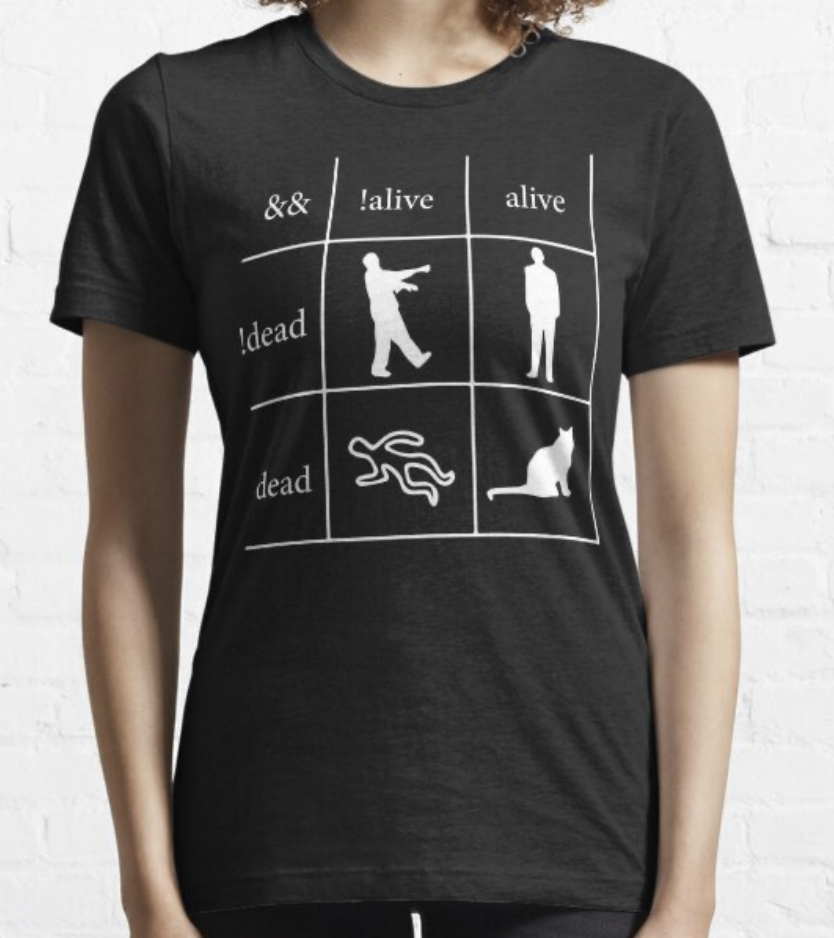
\includegraphics[height=\paperheight]{meme-modelo-booleano.png}
	
	\end{frame}
		
	%------------------------------------------------
	% Duda para introducir el Modelo Vectorial
	\begin{frame}
		
		\frametitle{Duda}
		
		\noindent\begin{minipage}{.4\textwidth}
			
			\textcolor{purple}{¿Puede obtenerse un ranking sobre el conjunto de datos según el nivel de pertenencia o similitud que tiene cada dato con una consulta?} 
			
			\only<2>{
				\vspace{2\baselineskip}
				R/:Sí, usando el Modelo Vectorial como primera aproximación.
			}
			
		\end{minipage}%
		\begin{minipage}{.7\textwidth}
			\centering
			
\includegraphics[scale=0.36]{duda.png} 
		\end{minipage}
		
	\end{frame}
	
	%------------------------------------------------
	% Modelo Vectorial de RI 
	\begin{frame}
		
		\frametitle{Modelo Vectorial de RI}
		
		Características:
		\begin{itemize}
			
			\item Aprovecha el Álgebra Vectorial para definir relaciones de semejanza entre las representaciones vectoriales de los datos. \\[2mm]
			
			\item La consulta se define en el lenguaje natural. \\[2mm]
			
			\item $w_{i, j} \in \mathbb{R}$, $w_{i, j} \geq 0$ \\[2mm]
			
			\item Cada documento y la consulta se representa por un vector numérico de pesos.
			
		\end{itemize}
		
	\end{frame}
	
	%------------------------------------------------
	% Modelo Vectorial de RI 
	\begin{frame}
		
		\frametitle{Modelo Vectorial de RI}
		
		Ideas fundamentales:
		\begin{enumerate}
			
			\item Un término que aparece en muchos documentos \textbf{no debe} ser más importante que otro que aparece en pocos documentos. \\[2mm]
			
			\item Un documento con muchas ocurrencias de un término \textbf{no debe} considerarse menos importante que un documento con pocas ocurrencias de ese término.
			
		\end{enumerate}
		
	\end{frame}
	
	%------------------------------------------------
	% Modelo Vectorial de RI
	\begin{frame}
		
		\frametitle{Modelo Vectorial de RI}
		
		Se utiliza la función de similitud coseno para establecer la similitud entre un documento y la consulta.
		
		\begin{minipage}{.4\textwidth}
			
			\begin{align*}
				\hspace{1cm} sim(d_j, q) &= \frac{\overrightarrow{d_j} \cdot \overrightarrow{q}}{|\overrightarrow{d_j|} \cdot |\overrightarrow{q}|} \\
				 &= \frac{\sum_{i=1}^{n} w_{i, j} \times w_{i, q}}{\sqrt{\sum_{i=1}^{n} w_{i, j}^2} \times \sqrt{\sum_{i=1}^{n} w_{i, q}^2}}
			\end{align*}
			
		\end{minipage}%
		\begin{minipage}{.7\textwidth}
		
			\vspace{1\baselineskip}
			\centering
			\begin{tikzpicture}
				% Coordenadas de los vértices del triángulo
				\coordinate (A) at (0,0);
				\coordinate (B) at (3,0);
				\coordinate (C) at (2,2);
				
				% Dibujar los lados del triángulo
				\draw[->] (A) -- node[below] {$\overrightarrow{q}$} (B);
				\draw[->]  (A) -- node[above left] {$\overrightarrow{d_j}$} (C);
				
				% Etiquetar el ángulo
				\draw (1,0) arc (0:45:1);
				\node at (1.2,0.4) {$\theta$};
			\end{tikzpicture}
			
			$cos \ \theta \in [-1, 1]$
			
		\end{minipage}
		
		\pause
		\vspace{3\baselineskip}
		\textcolor{purple}{¿Pero cómo se computa el peso de cada término indexado en el documento?}
		
	\end{frame}
	
	%------------------------------------------------
	% Cálculo de los pesos en los documentos: tf
	\begin{frame}
		
		\frametitle{Cálculo de los pesos en los documentos}
		
		La frecuencia normalizada del término $t_i$ en el documento $d_j$ se define como: 
		
		$$tf_{i, j} = \frac{freq_{i, j}}{max_l freq_{l,j}} = \alpha + (1 - \alpha) \times  \frac{freq_{i, j}}{max_l freq_{l,j}}$$ 
		
		donde:
		\begin{itemize}
			
			\item $freq_{i, j}$ : frecuencia del término $t_i$ en el documento $d_j$
			
			\item $max_l freq_{l,j}$ : mayor frecuencia de todos los términos de $d_j$
			
			\item $\alpha$ $(\alpha \in [0, 1])$ : término de suavizado y permite amortiguar la contribución de la frecuencia del término. Los valores más usados son $0.4$ y $0.5$.
			
		\end{itemize}
		
		\vspace{2\baselineskip}
		
		Si $t_i \notin d_j$ entonces $tf_{i, j} = 0$.
		
	\end{frame}
	
	%------------------------------------------------
	% Cálculo de los pesos en los documentos: idf
	\begin{frame}
		
		\frametitle{Cálculo de los pesos en los documentos}
		
		La frecuencia de ocurrencia de un término $t_i$ dentro del conjunto de datos se define como:
		
		$$idf_i = \log \frac{N}{n_i}$$
		
		donde:
		\begin{itemize}
			
			\item $N$ : cantidad de documentos dentro del corpus
			
			\item $n_i$ : cantidad de documentos en los que aparece el término $t_i$ 
			
		\end{itemize}
		
		\pause
		\vspace{2\baselineskip}
		
		Luego, el peso de un término $t_i$ en un documento o la consulta $d_j$ está dado por:
		$$w_{i, j} = tf_{i, j} \times idf_{i}$$
		
		% Esta experesion da mayor valor a aquellos términos raros o pocos frecuentes y da valores ínfimos a aquellos términos que aparecen en todos los documentos.
		
	\end{frame}
	
	%------------------------------------------------
	% Definición formal del Modelo Vectorial de RI
	\begin{frame}
		
		\frametitle{Definición formal del Modelo Vectorial de RI}
		
		\begin{itemize}
			
			\item[] \textbf{D}: Vectores de pesos no binarios asociados a los términos de los documentos \\[2mm]
			
			\item[] \textbf{Q}: Vectores de pesos no binarios asociados a los términos de la consulta \\[2mm]
			
			\item[] \textbf{F}: Espacio $n$-dimensional y operaciones entre vectores del Álgebra Lineal \\[2mm]
			
			\item[] \textbf{R}: $sim(d_j, q) = \frac{\sum_{i=1}^{n} w_{i, j} \times w_{i, q}}{\sqrt{\sum_{i=1}^{n} w_{i, j}^2} \times \sqrt{\sum_{i=1}^{n} w_{i, q}^2}}$ 
			
		\end{itemize}
		
	\end{frame}
	
	%------------------------------------------------
	% Ventajas y desventajas del Modelo Vectorial
	\begin{frame}
		
		\frametitle{Ventajas y desventajas del Modelo Vectorial}
		
		Ventajas:
		\begin{itemize}
			
			\item Permite ordenar los documentos según el grado de similitud con la consulta.
			
			\item La estrategia de coincidencia parcial permite la recuperación de documentos que se aproximen a los requerimientos de la consulta.
			
			\item El esquema de ponderación mejora el rendimiento de la recuperación de los documentos.
			
		\end{itemize}
		
		\vspace{2\baselineskip}
		
		\pause 
		
		Desventajas:
		\begin{itemize}
			
			\item Asume que los términos indexados son mutuamente independientes.
			% Consecuencias:
			% 	- Pérdida de información contextual
			% 	- Ignora la estructura del lenguaje
			% 	- No considera la co-ocurrencia de términos
			% 	- Vulnerabilidad a la dimensionalidad
			
		\end{itemize}
		
	\end{frame}
	
	%------------------------------------------------
	% Break
	{
		\setbeamertemplate{background canvas}
		{%
			
\includegraphics[width=\paperwidth,height=\paperheight]{baile.png}
		}
		
		\begin{frame}
		\end{frame}
	}
	
	%------------------------------------------------
	% Modelo Probabilístico de RI
	\begin{frame}
		
		\frametitle{Modelo Probabilístico de RI}
		
		Características:
		\begin{itemize}
			
			\item El modelo intenta resolver el problema de la recuperación de información desde las probabilidades. \\[2mm]
			
			\item $w_{i, j} \in {0, 1}$ \\[2mm]
			
			\item El modelo intenta calcular la probabilidad en el que un documento sea relevante para una consulta realizada.
			% o sea, intenta estimar la probabilidad de que el usuario encuentre interesante el documento. \\[2mm]
			
			\item Existe un subconjunto de todos los datos que el usuario ``prefiere'' como respuesta a la consulta y el modelo debe de maximizar la relevancia de la información esperada por el usuario. \\[2mm]
			
			\item La probabilidad de relevancia depende únicamente de la representación de un documento y la consulta. 
			
		\end{itemize}
		
	\end{frame}
	
	%------------------------------------------------
	% Nociones de probabilidad
	\begin{frame}
		
		\frametitle{Nociones de probabilidad}
		
		Sean los eventos $A$ y $B$ entonces: \\
		\hspace{5.3cm} $p(A, B) = p(A \cap B) = p(A|B)p(B) = p(B|A)p(A)$
		
		\vspace{2\baselineskip}
		
		Teorema de Bayes: \\
		\hspace{3cm} $p(A|B) = \frac{p(B|A)p(A)}{p(B)}$
		
		% El teorema de Bayes es especialmente útil cuando queremos actualizar nuestras creencias sobre la ocurrencia de un evento A dado cierta evidencia B.
		% Se utiliza para inferir modelos probabilísticos y realizar inferencias basadas en datos observados.
		
		\vspace{3\baselineskip}
		
		Razón de probabilidades: \\
		\hspace{4cm} $O = \frac{p(A|B)}{p(\overline{A}|B)}$
		
		% Es una medida de la fuerza de asociación entre dos eventos. 
		% Es una proporción de probabilidad.
		% Es una medida útil para evaluar la asociación entre dos variables binarias.
		
	\end{frame}
	
	%------------------------------------------------
	% Modelo Probabilístico de RI
	\begin{frame}
		
		\frametitle{Modelo Probabilístico de RI}
		
		Para calcular la similitud se define la función:
		$$sim(d_j, q) = O(R|dj) = \frac{p(d_j \text{\ sea relevante})}{p(d_j \text{\ no sea relevante})}$$
		
		donde $R$ es la relevancia del documento con respecto a la consulta.
		
		\pause
		\vspace{2\baselineskip}
		
		Para poder computar la razón se usa:
		\begin{itemize}
			\item el Principio del Ranking Probabilístico, 
			\item el Teorema de Bayes, y
			\item la información de ocurrencia de los términos de la consulta en el documento.
		\end{itemize}
		
	\end{frame}
	
	%------------------------------------------------
	% Principio del Ranking Probabilístico
	\begin{frame}
		
		\frametitle{Principio del Ranking Probabilístico}
		
		\only<1>{
			\begin{alertblock}{}
				Si en un SRI la respuesta a una consulta es un ranking de los documentos de la colección en orden decreciente de probabilidad de relevancia y las probabilidades son estimadas con la mayor precisión basándose en los datos disponibles del sistema, la efectividad general de la respuesta respecto al usuario será la mayor que se puede obtener a partir de los datos.
			\end{alertblock}
		}
		
		\only<2->{
			Aplicando el teorema de Bayes sobre la función de similitud, se obtiene:
			$$sim(d_j, q) = \frac{p(d_j|R)p(R)}{p(d_j|\overline{R})p(\overline{R})}$$
			
			donde:
			\begin{itemize}
				\item $p(R)$: probabilidad de ser relevante el documento recuperado
				\item $p(\overline{R})$: probabilidad de no ser relevante el documento recuperado
				\item $p(d_j|R)$: probabilidad de que si se recupera un documento relevante sea $d_j$
				\item $p(d_j|\overline{R})$: probabilidad de que si no se recupera un documento relevante sea $d_j$
			\end{itemize}
		}
		
		\only<3>{
			\vspace{2\baselineskip}
			\textcolor{black}{Como no se conocen las probabilidades a priori, es necesario estimar los valores usando el \textbf{Modelo de Independencia Binaria}.}
		}
		
	\end{frame}
	
	%------------------------------------------------
	% Modelo de Independencia Binaria
	\begin{frame}
		
		\frametitle{Modelo de Independencia Binaria}
		
		Permite calcular las probabilidades en la función de similitud, teniendo en cuenta las siguientes consideraciones:
		
		\begin{itemize}
			
			\item Lo documentos son representados como vectores binarios de términos. (Modelo de Independencia \textbf{Binaria}) \\[2mm]
			
			\item Se asume que los términos ocurren de manera independiente en los documentos. (Modelo de \textbf{Independencia} Binaria) \\[2mm]
			
			\item Documentos distintos pueden ser modelados como un mismo vector. \\[2mm]
			
			\item Solo interesa realizar una ordenación por relevancia de los datos.
			
		\end{itemize}
		
	\end{frame}
	
	%------------------------------------------------
	% Modelo de Independencia Binaria
	\begin{frame}
		
		\frametitle{Modelo de Independencia Binaria}
		
		\begin{align*}
			\only<1-4>{
				sim(d_j, q) &= O(R|\overrightarrow{d_j}) \\
			}
			\only<1-2>{
				&= \frac{p(\overrightarrow{d_j}|R)p(R)}{p(\overrightarrow{d_j}|\overline{R})p(\overline{R})} \quad \text{Aplicado el Teorema de Bayes} \\
				&= \frac{p(R)}{p(\overline{R})} \times \frac{p(\overrightarrow{d_j}|R)}{p(\overrightarrow{d_j}|\overline{R})}
			}
			\only<3-4>{
				&\approx \frac{p(\overrightarrow{d_j}|R)}{p(\overrightarrow{d_j}|\overline{R})} \\
				&\text{Asumiendo independencia entre los términos}  \\
				&\approx \frac{
						(\prod_{g_i(\overrightarrow{d_j}) = 1} p(t_i = 1|R)) \times (\prod_{g_i(\overrightarrow{d_j}) = 0} p(t_i=1|R))
					}{
						(\prod_{g_i(\overrightarrow{d_j}) = 1} p(t_i = 0|\overline{R})) \times (\prod_{g_i(\overrightarrow{d_j}) = 0} p(t_i = 0|\overline{R}))		
					}\\
			}
			\only<4>{
				&\text{Si $p(t_i = 1|R) + p(t_i = 0|R) = 1$ y se ignora factores contantes}  \\
				sim(d_j, q) &\approx \sum_{i = 1}^{n} w_{i, q} \times w_{i, j} \times (\log \frac{p(t_i|R)}{1 - p(t_i|R)} + \log \frac{1 - p(t_i|\overline{R})}{p(t_i|\overline{R})}) \\
			}
			\only<5>{
			sim(d_j, q) &\approx \sum_{i = 1}^{n} w_{i, q} \times w_{i, j} \times (\log \frac{p(t_i|R)}{1 - p(t_i|R)} + \log \frac{1 - p(t_i|\overline{R})}{p(t_i|\overline{R})})
			}
		\end{align*}
		
		\begin{tikzpicture}[remember picture,overlay]
			
			\only<2>{
				% Cuadro Azul
				\draw[draw=blue] (5.1,0.23) rectangle (5.95,1.43);
				\node[draw=blue,fill=blue!20,rectangle,rounded corners=3pt,inner sep=5pt,text width=4cm] (box1) at (2.5,-1) {\begin{minipage}{\textwidth}Valor constante para todos los documentos \\ dada una consulta\end{minipage}};
				\draw[->,blue,thick] (box1.east) to[out=0,in=270] (5.5,0.2);
				
				% Cuadro Rojo
				\draw[draw=red] (6.35,0.23) rectangle (7.7,1.48);
				\node[draw=red,fill=red!20,rectangle,rounded corners=3pt,inner sep=5pt] (box2) at (9.8,-0.8) {Término a estimar};
				\draw[->,red,thick] (box2.west) to[out=180,in=270] (7,0.2);
			}
			
			\only<4>{
				% Cuadro Azul
				\draw[draw=orange] (2,1.15) rectangle (12,2.36);
			}
			
		\end{tikzpicture}
	
		\only<3>{
			Donde:
			\begin{itemize}
				\item $t_i = 1$: significa que el término $t_i$ ocurre en el documento $d$
				\item $t_i = 0$: significa que el término $t_i$ no ocurre en el documento $d$
			\end{itemize}
		}
	
		\only<5>{
			Donde:
			\begin{itemize}
				\item $p(t_i|R) = 0.5$
				\item $p(t_i|\overline{R}) = \frac{n_i}{N}$ \\[3mm]
			\end{itemize}
			
			Estos valores son aproximaciones iniciales, las cuales tienen forma de ajustarse al conjunto de datos del sistema (ver en clase posterior).
		}
		
	\end{frame}
	
	%------------------------------------------------
	% Definición formal del Modelo Probabilístico de RI
	\begin{frame}
		
		\frametitle{Definición formal del Modelo Probabilístico de RI}
		
			\begin{itemize}
				
				\item[] \textbf{D}: Vectores de pesos binarios asociados a los términos de los documentos \\[2mm]
				
				\item[] \textbf{Q}: Vectores de pesos binarios asociados a los términos de la consulta \\[2mm]
				
				\item[] \textbf{F}: Teoría de Probabilidades \\[2mm]
				
				\item[] \textbf{R}: $sim(d_j, q) = O(R|dj) = \frac{p(d_j \text{\ sea relevante})}{p(d_j \text{\ no sea relevante})}$
				
			\end{itemize}
		
	\end{frame}
	
	%------------------------------------------------
	% Ventajas y desventajas del Modelo Probabilístico
	\begin{frame}
		
		\frametitle{Ventajas y desventajas del Modelo Probabilístico}
		
		Ventajas:
		\begin{itemize}
			
			\item Permite obtener un ranking entre los documentos recuperados.
			
		\end{itemize}
		
		\vspace{2\baselineskip}
		
		\pause 
		
		Desventajas:
		\begin{itemize}
			
			\item El peso de los términos es binario, por lo que no se considera la frecuencia de ocurrencia de los mismos.
			
			\item Se asumen independencia entre los términos.
			% No siempre la independencia de los términos es una mala suposición en situaciones práctica. El modelo Naive Bayes es muy bueno porque tiene esta consideración.
			
			\item Es necesario encontrar un primer conjunto de documentos relevantes para los valores particulares de $p(t_i|R)$ y $p(t_i|\overline{R})$.
			
		\end{itemize}
		
	\end{frame}
	
	%------------------------------------------------
	% Break
	{
		\setbeamertemplate{background canvas}
		{%
			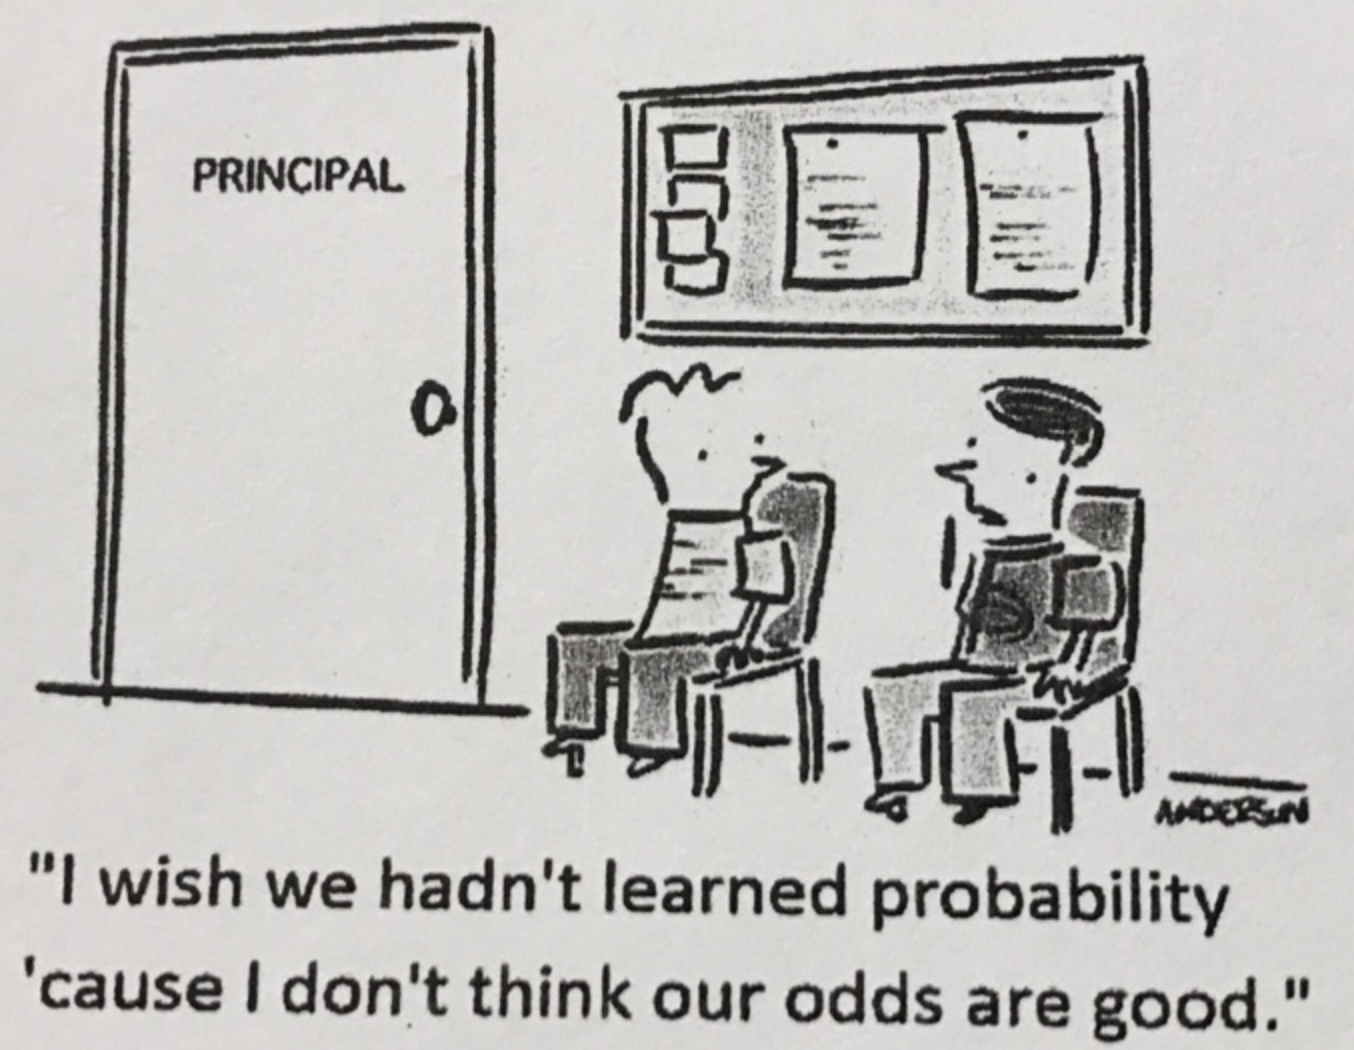
\includegraphics[width=\paperwidth,height=\paperheight]{break-3.png}
		}
		
		\begin{frame}
		\end{frame}
	}
	
	%------------------------------------------------
	% Comparación entre los modelos clásicos
	\begin{frame}
		
		\frametitle{Comparación entre los modelos clásicos}
		
			\begin{table}[h]
			\centering
			\begin{tabular}{|p{3cm}|p{3cm}|p{3.7cm}|p{3.3cm}|}
				\hline
				\textbf{Criterios} & \textbf{Booleano} & \textbf{Vectorial} & \textbf{Probabilístico} \\
				\hline
				\hline
				Documentos& Vectores binarios & Vectores reales & Vectores binarios \\
				\hline
				Consultas & Expresión booleana & Vector real &Vector binario \\
				\hline
				Framework & Teoría de Conjuntos y Álgebra Booleana & Espacio $n$-dimensional y operaciones entre vectores del Álgebra Lineal & Teoría de Probabilidad \\
				\hline
				Pesos & Binario & Real & Binario \\
				\hline
				Similitud & {0, 1} & Dada por el coseno del ángulo entre el documento y la consulta & Dada por la probabilidad de que el documento sea relevante a la consulta \\
				\hline
				Dependencia entre los términos & No & No & No \\
				\hline
				Correspondencia parcial documento-consulta & No & Sí & Sí \\
				\hline
				Ranking & No & Sí & Sí \\
				\hline
			\end{tabular}
		\end{table}
		
	\end{frame}
	
	%------------------------------------------------
	% Conclusiones
	\begin{frame}
		
		\frametitle{Conclusiones}
		
		\begin{itemize}
			
			\item Se considera que el MRI Booleano es el más débil y su problema principal es la incapacidad para reconocer coincidencias parciales. No obstante es rápido.
			
			\item El MRI Vectorial es simple y en algunos casos brinda mejores resultados en la RI que el resto de los MRI clásicos. \\[2mm]
			
			\item El MRI Probabilístico ofrece una recuperación adecuada, sin embargo, experimentos han demostrado que el MRI Vectorial es el que tiene el mejor desempeño. Además, es compleja su implementación.
			
		\end{itemize}
		
	\end{frame}
	
	%------------------------------------------------
	% Bibliografía
	\begin{frame}
		
		\frametitle{Bibliografía}
		
		\begin{itemize}
			\item Baeza-Yates, R. a.-N. (2002). Modern Information Retrieval. Capítulo 2.
			\item Manning, C. D. (2009). An Introduction to Information Retrieval . Cambridge UP. Capítulos 1, 4-6, 11.
			\item Baeza-Yates, R. a. (s.f.). Information Retrieval: Data Structures \& Algorithms, Capítulo 3.
		\end{itemize}
		
	\end{frame}
	
	%------------------------------------------------
	% Fin
	\begin{frame}
		\titlepage
	\end{frame}
	
	
	
\end{document} 